\documentclass[]{article}
\usepackage{multirow, listings, pgfplots, tablefootnote, amsmath, float, graphicx}%multirow for tables, listings to import python code, pgfplots to plots data, tablefootnote for notes under a table, amsmath for equations (as fraction case for probability),
                                                                        %float for text under table, graphicx to scale tables
\usepackage[]{}
\pgfplotsset{width = 10cm, compat = 1.9}

\begin{document}


\title{\textbf{Alberi Rosso-Neri vs Alberi Binari di Ricerca}}
\author{Assioma Andrea Aligi}
\date{13 Gennaio 2022}
\maketitle

{\Large \textbf{1. Introduzione}}\\
Nella seguente relazione si vuole analizzare le differenze tra Alberi Binari di Ricerca e Alberi Rosso-Neri, 
in particolare come variano i tempi medi di ricerca degli elementi inseriti, a seconda del tipo di lista. \\
\\
Gli Alberi Binari di Ricerca (ABR) e gli Alberi Rosso-Neri (ARN) sono strutture dati collegate caratterizzate da:
\begin{itemize}
    \item \textbf{T.root} un puntatore a alla radice dell'albero.
    \item \textbf{x.p} un puntatore al padre del nodo x.
    \item \textbf{x.left} un puntatore al successivo nodo sinistro (è quindi il figlio sinistro del nodo x).
    \item \textbf{x.right} un puntatore al successivo nodo destro(è il figlio destro del nodo x).
    \item \textbf{x.key} un attributo che aggiunge al nodo x un valore chiamato chiave.
\end{itemize}
L'Albero Rosso-Nero, rispetto all'Albero Binario di Ricerca, possiede anche un attributo chiamato colore (\textbf{x.color}) che può essere rosso o nero, e le sue foglie non contengono valore.\\
\\
Entrambi gli alberi supportano operazioni dinamiche, tra cui l'inserimento e la ricerca.\\
L'algoritmo di ricerca ritorna il tempo che impiega per individuare un nodo (generalmente \textit{O}(lg\textit{n})), se esiste. Altrimenti, ritorna un valore vuoto NIL.\\
L'algoritmo di inserimento, invece, aggiunge un nuovo nodo all'interno di un albero dato in input, scorrendo tra quelli già inseiriti. 
Nel caso degli ARN gli viene attribuito anche un colore, 
e perciò necessita di un'ulteriore funzione la quale evita che vengano violate le 5 proprietà di questo tipo di albero.\\

\newpage
{\Large \textbf{{\Large{1}}.{\small{1}}. Hardware e Sistema operativo utilizzati}}\\
Le piattaforme su cui verranno effettuati gli esperimenti sono:
\begin{itemize}
  \item Un pc fisso con processore i5-10600k e 16gb di ram. Il sistema operativo adoperato è Ubuntu 20.04..
  \item Un portatile con processore M1 e 8 gb di ram. Il sistema operativo adoperato è OS Monterey.
\end{itemize}
Non in tutti gli esperimenti sono stati usati entrambi.\\

{\Large \textbf{2. Algoritmo di ricerca}}\\
In generale, è difficile stabilire un tempo medio per quanto riguarda le operazioni di ricerca degli elementi in un albero, 
in quanto quest'ultimo non è sempre uguale. E' possibile comunque provare che la distanza media di un nodo a partire dalla radice è \textit{O}(lg\textit{n}), 
ed è quindi assimilabile a un'analisi del metodo di ricerca.\\
L'inserimento degli elementi della lista verrà effettuato in modo ricorsivo. 
Tali liste avranno dimensione 100, 250, 500, 800, 900, 100, 1250, 1500, 2000 e si distinguono in ordinate in modo crescente e casuali 
(cioè liste ordinate, i cui elementi sono stati "mescolati" in modo casuale tramite apposita funzione \texttt{random.sample()}).\\
Per ciascuna lista sono state effettuate 50 prove, e, successivamente, si è calcolata la media.\\
In python è stato imposto un limite di ricorsioni per evitare l'overflow dello stack e per buona pratica di programmazione si evita di aumentare tale limite:
perciò gli elementi della lista sono stati inseriti in modo iterativo.\\
Prima dell'analisi dei risultati, ci si può aspettare che nel caso dell'Albero Binario di Ricerca si avrà una distanza media di un nodo dalla radice più elevata, 
specialmente nell'inserimento di liste ordinate (in quanto si sta praticamente realizzando un albero con altezza massima \texttt{n}-1, dove \texttt{n} rappresenta la lunghezza della lista inserita).\\
Nel caso degli Alberi Rosso-Neri, invece, ci si può aspettare delle distanze medie minori grazie all'implementazione del metodo \texttt{insertFixup}, 
il quale "bilancia" l'albero in modo tale che, nel momento in cui si cerca un nodo, non si scende troppo in profondità.\\ 
Per entrambi gli algoritmi sono state realizzate delle funzioni iterative di inserimento e in ARN è stata usata una funzione iterativa di ricerca degli elementi per il calcolo della distanza di ogni nodo dalla radice.\\
In ABR, invece, la distanza è stata calcolata direttamente all'interno del metodo di inserimento in quanto è risulato più semplice e pratico 
\\(\texttt{nodeInsertion} ha implementazione simile a quella del metodo di ricerca, e quindi non presenta una chiamata alla funzione \texttt{insertFixup}, come nel caso degli ARN).\\

\newpage
{\large \textbf{{\Large{2}}.{\small{1}}. Albero binario di ricerca}}\\
Per l'implementazione del seguente tipo di albero, sono state realizzate due classi:
\begin{itemize}
    \item \texttt{Node}: è una classe che possiede solo il costruttore e nessun altro metodo. Permette di realizzare il nodo di un albero che ha come attributi un valore chiamato chiave (key) e due puntatori ai figli.\\
          Ogni volta che viene istanziato un suo oggetto:
          \begin{itemize}
            \item I figli \texttt{self.left} e \texttt{self.right} sono inizializzati a \texttt{None} (vuoti).
            \item L'attributo \texttt{key}, assume il valore dato in input.
          \end{itemize}  
    \item \texttt{BST}: è la classe che inizializza e sviluppa l'albero, e calcola la distanza di un nodo dalla radice. I metodi utilizzati sono:
          \begin{itemize}
            \item \texttt{setRoot} inizializza il nodo radice, prendendo il primo nodo inserito come input. Questo metodo è utile per puntare alla radice dell'ablero.
            \item \texttt{insert} permette l'inserimento di un nodo, sia questo il primo (e quindi il nodo radice) o uno successivo. Come input prende solo il valore (\texttt{key}) da assegnare al nodo.
            \item \texttt{nodeInsertion} permette l'inserimento di nodi successivi a quello radice. Inoltre, calcola la distanza del nodo inserito a partire dalla radice. 
                  Come input si ha il nodo di partenza e la chiave da inserire. Come output, si ha la distanza espressa in numero di nodi "attraversati" durante l'inserimento.
          \end{itemize}  
\end{itemize}
\newpage
L'esito degli esperimenti è stato il seguente (con valori espressi a tre cifre significative):\\ 

\begin{table}[H]
  \makebox[\linewidth]{
  \resizebox{13cm}{!}{
  \begin{tabular}{||c|cccccccccc||}
    \hline
    \multicolumn{1}{|c|}{} & \multicolumn{10}{|c|}{Lunghezze liste}\\
    \hline
    \multicolumn{1}{|c|}{Tipo di Lista} & \multicolumn{10}{|c|}{Risultati}\\
    \hline\hline
    Lista Ordinata & 100 & 250 & 500 & 800 & 900 & 1000 & 1250 & 1500 & 1750 & 2000 \\
    \hline\hline
    Tempo medio in 50 run & 49.5 & 125 & 250 & 399.5 & 450 & 500 & 625 & 750 & 875 & 1000\\
    \hline\hline
    Lista Casuale & 100 & 250 & 500 & 800 & 900 & 1000 & 1250 & 1500 & 1750 & 2000 \\
    \hline\hline
    Tempo medio in 50 run & 6.49 & 8.23 & 9.55 & 10.4 & 10.9 & 11.0 & 11.3 & 11.7 & 12.1 & 12.4\\
    \hline
  \end{tabular}
  }
  }  
  {\footnotesize{\textbf{Il tempo di inserimento di una lista è espresso in numero di nodi.}}}
\end{table}

A livello grafico si ha invece:
\begin{center}
  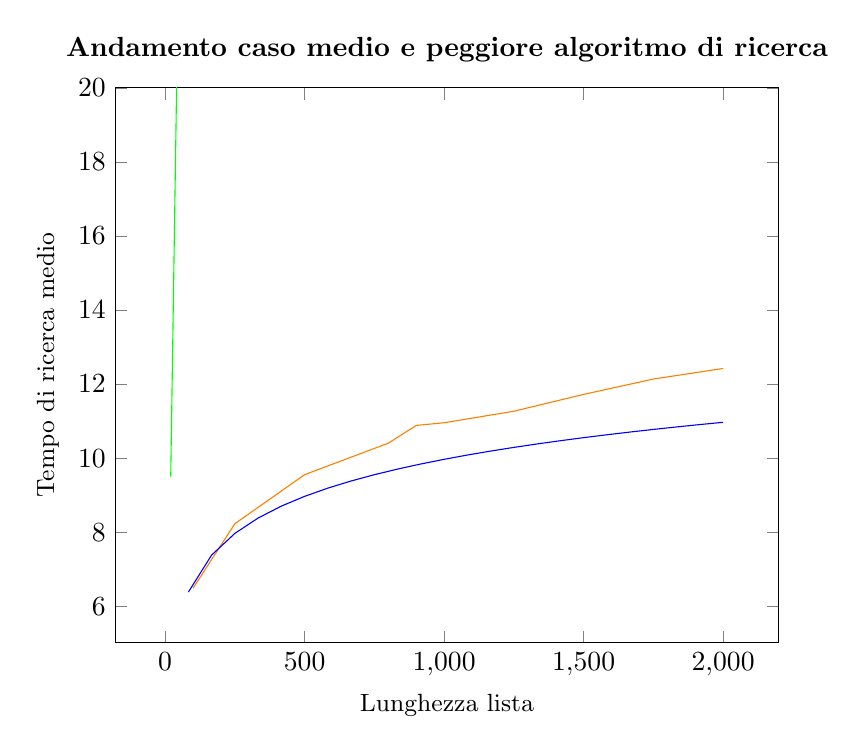
\begin{tikzpicture}
    \begin{axis}[title = {\textbf{Andamento caso medio e peggiore algoritmo di ricerca}},
      xlabel = \small{Lunghezza lista}, ylabel =\small{Tempo di ricerca medio}, scaled y ticks = false, scaled x ticks = false, ymax = 20]
      \addplot[color = green] coordinates{(20, 9.5)(100, 49.5)(250, 124.5)(500, 249.5)(800, 399.5)(900, 449.5)(1000, 499.5)(1250, 624.5)(1500, 749.5)(1750, 874.5)(2000, 999.5)};
      \addplot[color = orange] coordinates{(100, 6.4862)(250, 8.229)(500, 9.5532)(800, 10.4033)(900, 10.8828)(1000, 10.95468)(1250, 11.265984)(1500, 11.72072)(1750, 12.1354286)(2000, 12.42163)};
      \addplot[color = blue, domain = 0:2000] {ln(x)/ln(2)};
    \end{axis}
  \end{tikzpicture}
\end{center}

La funzione di inserimento di una lista casuale impiega generalmente meno tempo rispetto all'inserimento in ordine crescente.\\

{\large \textbf{{\Large{2}}.{\small{2}}. Albero rosso-nero}}\\
Ha implementazione simile all'albero binario di ricerca, con la differenza che vengono aggiunti due nuovi attributi (\texttt{color} e un puntatore al padre \texttt{p} ) 
e due nuovi metodi (uno che impedisce la violazione delle 5 proprietà dell'albero, l'altro, invece, ricerca un nodo a partire dalla radice per determinarne la distanza). 
Si hanno comunque due classi:\\
\begin{itemize}
  \item \texttt{Node}: simile alla classe dell'albero precedente, possiede un ulteriore l'attributo \texttt{color} e un puntatore al padre, dati in input dall'utente. 
  Nel momento in cui viene istanziato un oggetto, il valore \texttt{color} può essere "Red" o "Black".
  \item \texttt{RBT}: inizializza l'albero e inserisce nodi. \texttt{insert} e \texttt{nodeInsertion} sono praticamente invariati. Solo 
  \texttt{nodeInsertion} presenta una chiamata aggiuntiva a una nuova funzione posta successivamente all'inserimento del nuovo nodo, e cioè \texttt{insertFixup}.\\
  Presenta tre ulteriori metodi:
  \begin{itemize}
    \item \texttt{insertFixup} modifica la struttura dell'albero, attraverso rotazioni o il cambiamento di colore dei nodi, affinché non si violano proprietà dell'albero. Come input prende il nuovo nodo inserito
    \item \texttt{leftRotate} e \texttt{rightRotate} sono metodi che ruotano, rispettivamente, a sinistra e a destra un nodo dato in input.
    \item \texttt{searchNode} cerca il nodo dato in input a partire dalla radice, e ritorna in output la distanza da quest'ultima.
  \end{itemize}  
\end{itemize}
Gli esiti degli esperimenti sono stati effettuati con le stesse notazioni dell'albero precedente:
\begin{table}[H]
  \makebox[\linewidth]{
    \resizebox{13cm}{!}{
    \begin{tabular}{||c|cccccccccc||}
      \hline
      \multicolumn{1}{|c|}{} & \multicolumn{10}{|c|}{Lunghezze liste}\\
      \hline
      \multicolumn{1}{|c|}{Tipo di Lista} & \multicolumn{10}{|c|}{Risultati}\\
      \hline\hline
      Lista Ordinata & 100 & 250 & 500 & 800 & 900 & 1000 & 1250 & 1500 & 1750 & 2000 \\
      \hline\hline
      Tempo medio in 50 run & 5.30 &  6.42 & 7.42 & 8.14 & 8.18 & 8.41 & 8.89 &  8.93 & 9.33 & 9.40 \\
      \hline\hline
      Lista Casuale & 100 & 250 & 500 & 800 & 900 & 1000 & 1250 & 1500 & 1750 & 2000 \\
      \hline\hline
      Tempo medio in 50 run & 4.93 & 6.25 & 7.24 & 7.93 & 8.09 & 8.25 & 8.57 & 8.85 & 9.07 & 9.27 \\
      \hline
    \end{tabular}
    }
  }  
\end{table}
\newpage
A livello grafico si ha invece:
\begin{center}
  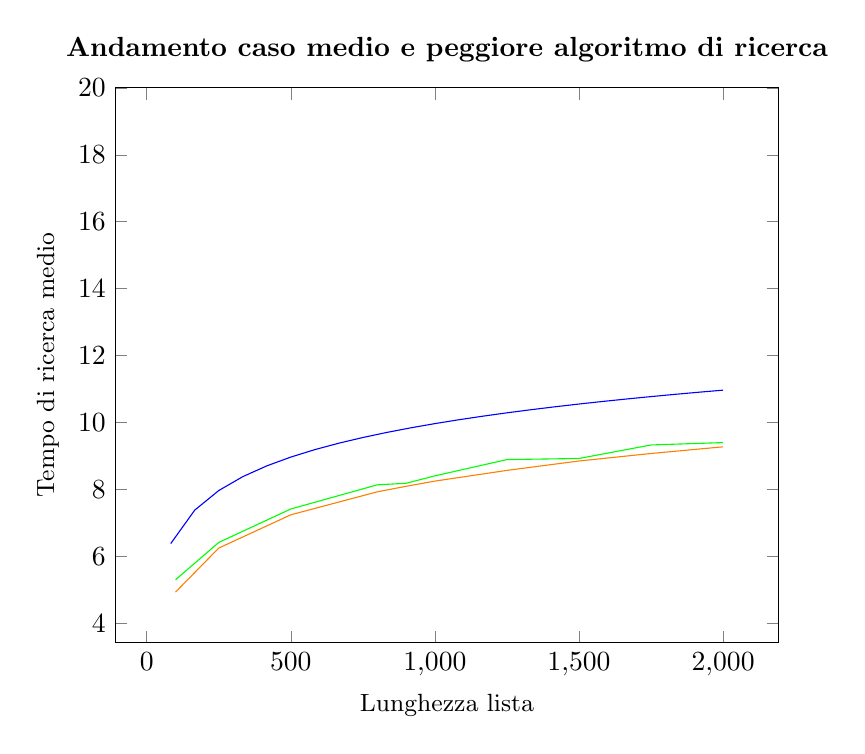
\begin{tikzpicture}
    \begin{axis}[title = {\textbf{Andamento caso medio e peggiore algoritmo di ricerca}},
      xlabel = \small{Lunghezza lista}, ylabel =\small{Tempo di ricerca medio}, scaled y ticks = false, scaled x ticks = false, ymax = 20]
      \addplot[color = green] coordinates{(100, 5.3)(250, 6.416)(500, 7.416)(800, 8.1375)(900, 8.184)(1000, 8.406)(1250, 8.892)(1500, 8.925)(1750, 9.329)(2000, 9.4)};
      \addplot[color = orange] coordinates{(100, 4.9332)(250, 6.248)(500, 7.2416)(800, 7.928625)(900, 8.09364)(1000, 8.24874)(1250, 8.569216)(1500, 8.850027)(1750, 9.07421714)(2000, 9.27341)};
      \addplot[color = blue, domain = 0:2000] {ln(x)/ln(2)};
    \end{axis}
  \end{tikzpicture}
\end{center}

Dalla tabella si può notare l'efficacia di \texttt{insertFixup}, il quale riduce di molto le distanze dei nodi dalla radice.\\

{\large \textbf{{\Large{2}}.{\small{3}}. Conclusioni}}\\
In entrambi gli alberi si può notare come il tempo medio di ricerca ha un andatura logaritmica, 
e quindi si "stabilizza" a partire dalle liste di lunghezza maggiore o uguale a 900.\\
Rispetto a quanto intuito preventivamente, nel caso del calcolo della profondità media di una lista casuale nell'Albero Binario di Ricerca non si ha esattamente 
\textit{O}(lg\textit{n}), ma si è molto vicini a tale stima: ciò può essere dovuto a una serie di casi sfortunati in cui la profondità è risultata molto più elevata e 
hanno fatto media con dei casi migliori.\\
Per il resto, non ci si è discostati molto dalle ipotesi iniziali: 
infatti, viene marcata la differenza dei tempi di ricerca nell'inserimento di una lista ordinata nell'Albero Binario di Ricerca rispetto ai restanti casi.

\end{document}